\graphicspath{{figures/chapter5/}}
\onehalfspacing

\chapter{Towards a low-cost multi-camera multi-epoch monitoring with deep learning photogrammetry}\label{ch:5}

\vfill

\newthought{This chapter is based on:}

\begin{itemize}
  \item AA
\end{itemize}

\newpage

\section{Introduction\textcolor{red}{TODO}}


\section{Image matching in challenging scenarios\textcolor{red}{TODO}}

Identifying homologous or tie points in pairs of images serves as the foundational task in photogrammetry for non-contact 3D measuring methods. These points allow for orienting single, stereo, or multi-image configurations. Applications span a wide range, depending by object size and the requisite level of accuracy, encompassing industrial, architectural, engineering, and remote sensing applications, requiring measurements on sparse control points or evaluations on dense reconstructions via multi-view dense image matching. Classical photogrammetric outputs include 3D point clouds, orthophotos, and digital surface models. [Other applications in CV, VO and SLAM] 

Historically, local image features (also keypoints or interest points), were initially identified manually, with automatic approaches emerging between the 1980s and the early 2000s. The evolution of these approaches spans a broad temporal spectrum (Figure 1), gradually identifying algorithms that effectively deal with those fundamental characteristics necessary for reliable image features (Lowe, 2004). Image detectors should identify repeatable keypoints across different images, described by a descriptor vector that characterizes the keypoint local neighborhood allowing for similarity matching across different image views. These detectors and descriptors should exhibit invariance to scale differences, arbitrary rotations, radiometric changes, and multi-view perspective projections. Moreover, descriptors should be distinctive and unambiguous.  

Several groundbreaking works emerged, significantly contributing to the proliferation and advancement of fully automatic structure-from-motion (SfM) software. Particularly noteworthy is SIFT (Scale Invariant Feature Transform), which, despite its acknowledged limited invariance to illumination and affine transformations (Lowe et al., 2004), marked a significant milestone as the first detector and descriptor demonstrating sufficient invariance for a broad spectrum of applications. Even today, SIFT remains the benchmark feature among non-deep learning-based approaches, often referred to as hand-crafted methods (Jin et al., 2021). 

Figure 1 illustrates a timeline of benchmark features. Initially, corner detectors were utilized in the early works (Harris and Stephen, 1988), transitioning to blob detectors that achieved a broader degree of scale and rotation invariance (Lowe, 1999; Lowe, 2004). Computational efficiency plays a pivotal role; for instance, SURF was developed with the explicit goal of improving upon SIFT computation time, whilst ORB was engineered as a binarized feature tailored for real-time applications. [Missing affine methods (both hand-crafted and DL), introduce machine-learning approaches before DL]. 

Since 2015, a novel category of deep-learning (DL) approaches has emerged to address the limitations of existing features. Initially, these methods involved independently training detectors and descriptors on extensive datasets comprising multi-temporal images, challenging illumination and perspective changes, and wide baselines (Verdie et al., 2015; Mishchuk et al., 2017; Barroso-Laguna et al., 2019). Subsequently, there has been a shift towards jointly training detectors and descriptors, starting with the seminal work of LIFT (Trulls et al., 2016), followed by other end-to-end DL approaches such as LF-Net (Ono et al., 2019), SuperPoint (DeTone et al., 2018), and ASLFeat (Luo et al., 2020). Generally, any combination of hand-crafted and DL approaches is feasible (Jin et al., 2021). 

Additionally, the matcher component can also be trained using DL techniques. A pioneering and groundbreaking approach in this regard was SuperGlue (Sarlin et al., 2020), which was followed by LightGlue (Lindenberger et al., 2023) and [expand]. Another dynamic category encompasses semi-dense matchers such as LoFTR (Sun et al., 2021) and RoMa (Edstedt et al., 2023b). However, it is noteworthy that they can identify tie points only on image pairs [expand]. 

[Add results from available paper that compares DL features] 

A limitation of deep learning (DL) local features is their limited invariance to rotation, due to training on images oriented almost upright. Although some authors initially emphasized this aspect, many approaches proposed in the literature do not prioritize it. For instance, LIFT and LFNet stand out as two examples of rotationally invariant end-to-end approaches, followed by RoRD (Parihar et al., 2021) and SE2-LoFTR (Bökman and Kahl, 2022) among semi-dense matchers. OriNet (Mishkin et al., 2018) becomes relevant when indipendent detectors and descriptors are combined (Bellavia et al., 2022). Recently, there has been renewed interest in addressing this limitation with the introduction of steerers [expand, citation + DeDoDe]. The relative lack of attention to rotation invariance may be attributed to a predominant focus in the computer vision community on datasets lacking extreme rotations (e.g., 90 and 180 degrees). Notably, in the Image Matching Challenge (IMC) from 2019 to 2022, datasets predominantly featured 'upright' images. However, the inclusion of rotated datasets in IMC 2023 highlighted a preference for using non-rotationally invariant descriptors, matching each image pair by rotating the second image by 90 degrees iteratively. This approach, however, proves computationally expensive when handling large datasets. 

Another limitation of DL approaches is their computational expense, rendering them unsuitable for deployment on full-resolution images, which are crucial for leveraging the available radiometric information in high-accuracy photogrammetric applications. In addition, it's worth noting that training itself often occurs on low-resolution images, a concern highlighted in [Ewelina paper], which impact remains uncertain. In fact, training could have generalized enough to do not require additional training on high resolution images [elaborate more]. 

While the potential of these approaches under extreme lighting conditions and radiometric variations is increasingly evident [add cit], some preliminary experiences suggest that these approaches may lack locally accurate identification, particularly in terms of the repeatability of keypoint positions [cit, also unsuperpoint]. 
Indeed, despite the existence of DL approaches for several years, their utilization in photogrammetric applications remains relatively limited. [Include relevant papers: satellite image analysis, glacier monitoring, and applications aimed at enhancing augmented reality (AR) and virtual reality (VR) experiences, coregistering laser scanner point clouds, Precision Agriculture Agriculture (Gao et al., 2024)]. 

The objective of this study is to assess the efficacy of DL local features for photogrammetric applications and introduce a novel DIM (Deep-Image-Matching) library to facilitate their adoption within the photogrammetric community. This library is designed to be compatible with various open-source and proprietary Structure-from-Motion (SfM) software. 

In comparison to existing literature, this work introduces several innovative aspects: 
\begin{itemize}
    \item Examination of DL local features' performance on high-resolution images. 
    \item  Addressing the challenge of managing rotations within the matching process. 
    \item Implementation of local refinement techniques to enhance feature matching accuracy. 
    \item Extension of semi-dense matchers, such as LoFTR and RoMa, to accommodate multi-view scenarios. 
    \item Evaluation of DL features on photogrammetric datasets to validate their suitability for real-world applications. 
    \item Introduction of a new evaluation metric, in addition to the conventional Root Mean Square Error (RMSE) assessment on checkpoint data. 
    \item Presentation of three additional applications showcasing the versatility of DL features (RGB to thermal image matching, ...). 
\end{itemize}

\begin{figure}
    \centering
    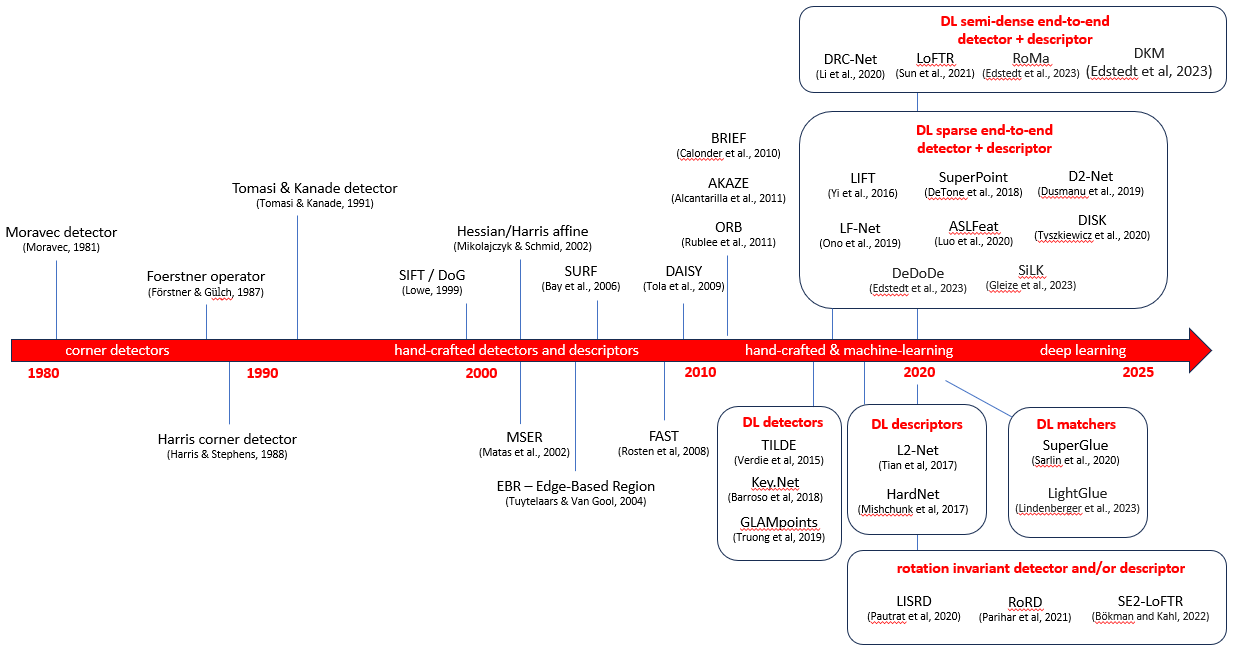
\includegraphics[width=1\textwidth]{local_feats_history}
    \caption{Timeline development of detectors, descriptors and matchers from preliminary works, hand-crafted, machine-learning, and deep-learning local features. (Cit.)}
    \label{fig:5:feats_history}
\end{figure}


\section{Deep-Image-Matching\textcolor{red}{TODO}}

Deep-Image-Matching (DIM) is a flexible, open-source Python library designed for robust multi-view image matching, leveraging both hand-crafted and DL matching techniques. DIM's primary goal is to provide a user-friendly interface to a wide selection of state-of-the-art computer vision algorithms for matching and tracking corresponding points across unordered images, providing the essential foundation for bundle adjustment and accurate photogrammetric reconstruction. 

Additionally, DIM aims at overcoming the main limitations of DL-based matching approaches that pose challenges for their practical usage in photogrammetry and remote sensing. These limitations include sensitivity to rotation changes, computational bottlenecks with high-resolution images (e.g., larger than 3000 px on the longest edge), difficulties in achieving sub-pixel accuracy, inefficient image pair selection for large datasets, and compatibility issues with existing SfM software packages.  

DIM itself does not perform the bundle adjustment and scene reconstruction, but it is designed to ensure seamless integration with various SfM packages, including COLMAP, OpenMVG, MicMac, and Agisoft Metashape, popular across the remote sensing and computer vision communities. This promotes workflow flexibility and interoperability across different pipelines. 

DIM employs a modular workflow designed for effective multi-view matching (Fig. XX).  

The process begins with a preprocessing stage where users select from different matching strategies (brute-force, low-resolution guided, sequential, image retrieval, or custom) to intelligently select the pair of images for optimized matching. Additionally, DIM provide a module for addressing the challenge of rotated images within datasets (e.g., in case of aerial or UAV surveys) by automatically identifying the ideal rotation angle between image pairs, significantly boosting matching accuracy. Users can opt to match images at their original resolution or employ down-sampling or up-sampling techniques managed by a quality parameter. To handle high-resolution imagery, DIM offers the added capability of image tiling, ensuring efficient processing without compromising detail. 

For the actual matching, DIM supports various combinations of local feature and matching algorithms, named pipelines, optimized for diverse problem domains. This allows users to tailor the workflow to their specific needs. Each pipeline consists of two main components: (I) an extraction Part that responsible for extracting local features from all images in the dataset; (ii) a matching Part that matches the extracted local features across the image pairs selected by the chosen matching strategy.  

DIM supports a wide range of local features and matching algorithms, spanning from the traditional ones to recent state-of-the-art learning approaches. Available local features include ORB, SIFT, SuperPoint (DeTone et al., 2020), ALIKE (Zhao et al., 2022), ALIKED (Zhao et al., 2023), DISK (Tyszkiewicz et al., 2020), Key.Net (Barroso-Laguna et al., 2019) + HardNet8 (Pultar, 2020), DeDoDe (Edstedt et al., 2023b). SuperGlue (Sarlin et al., 2020), LightGlue (Lindenberger et al., 2023), LoFTR (Sun et al., 2021), SE2-LoFTR (Bökman and Kahl, 2022), and RoMA (Edstedt et al., 2023a) are implemented as matchers. Additionally, KORNIA python library (Riba et al., 2020) can be used for nearest neighbor matching. 

A sub-pixel refinement module allows to improve the matching precision, expecially in case of DL-based features that works only at the pixel level. Robust geometric verification techniques then ensure the removal of inaccurate or unreliable matches. 

DIM efficiently stores extracted features—including their image coordinates, descriptors, and scores—in local HDF5 (Hierarchical Data Format¹) files using the h5py² library. Additionally, DIM creates a separate HDF5 file to store the indexes of matched features across all images. This indexing enables the construction of tracks, which build tracks of features matched across multiple images. Finally, DIM exports matched features in a variety of formats, ensuring compatibility with a wide range of popular SfM software packages. 

\begin{figure}
    \centering
    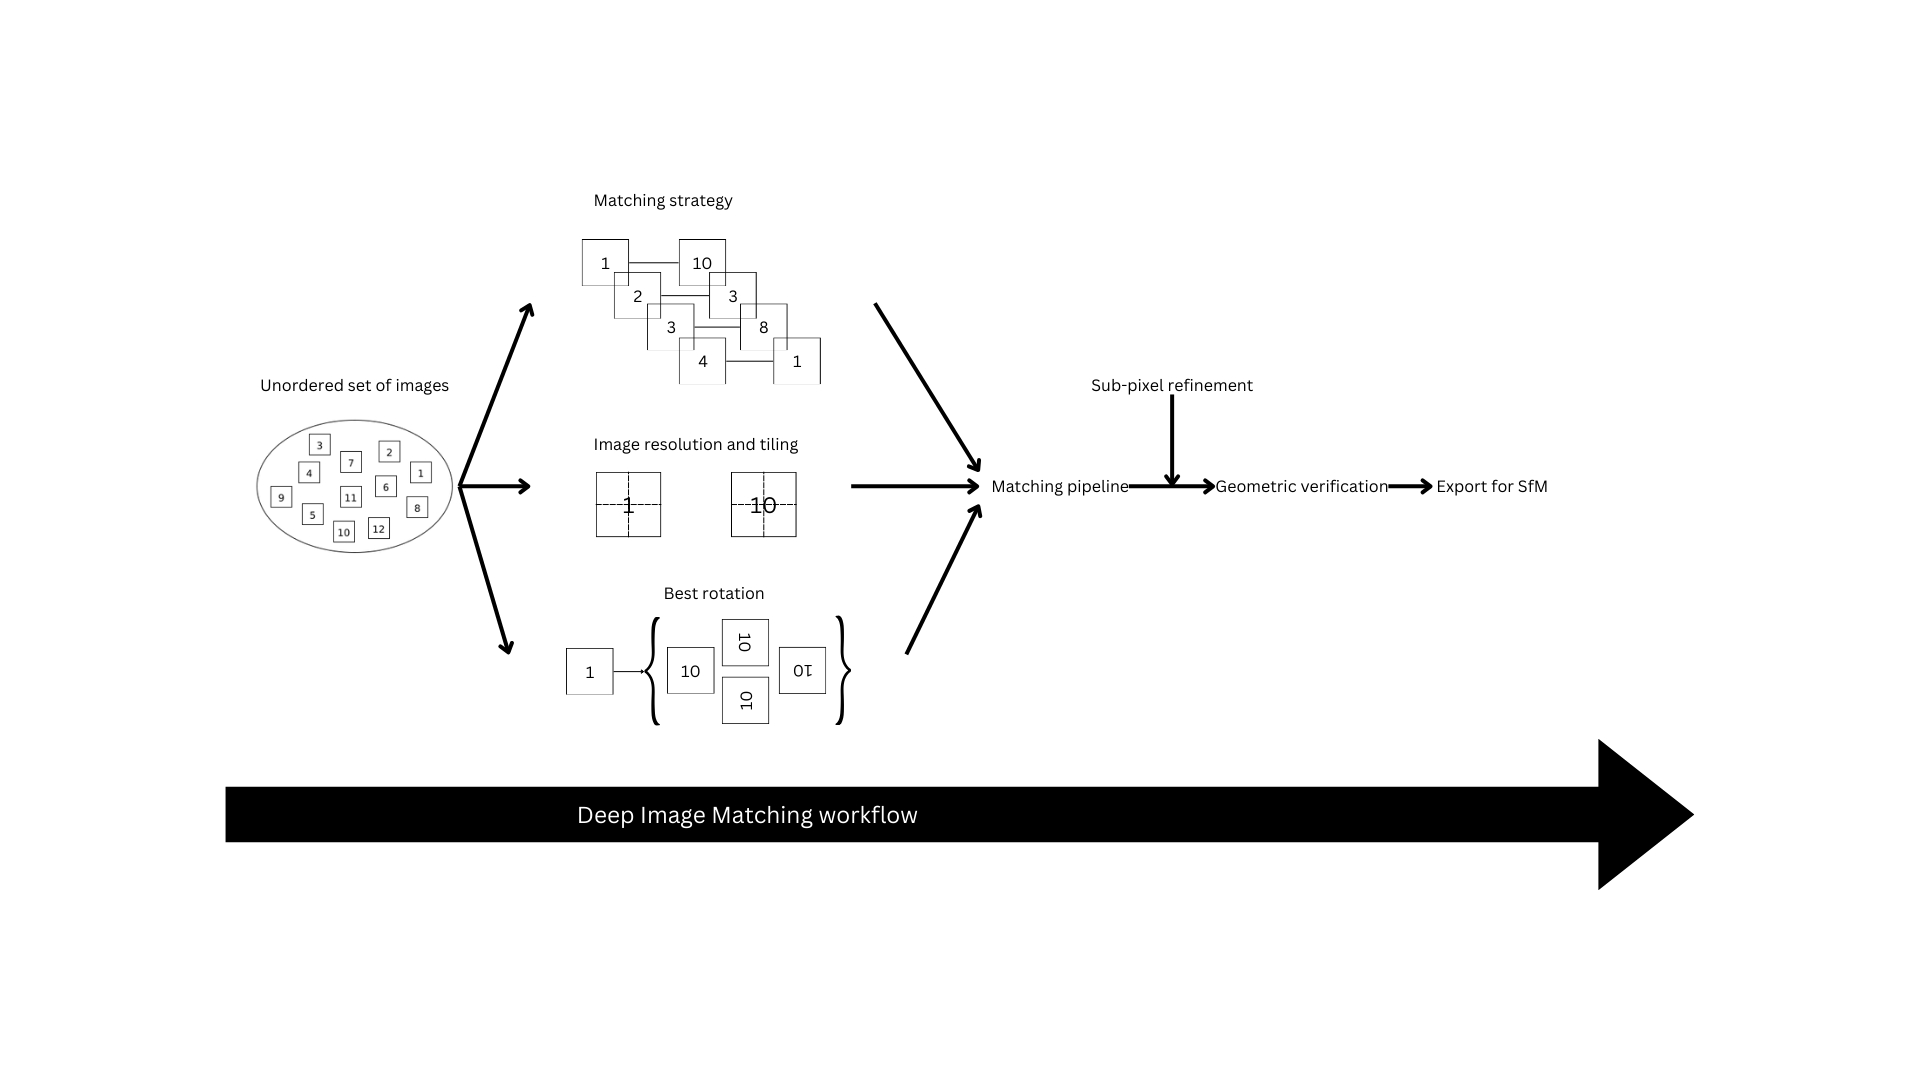
\includegraphics[width=1\textwidth]{dim_workflow}
    \caption{temporary DIM workflow}
    \label{fig:5:dim_workflow}
\end{figure}

\subsection{Matching strategies}

The matching strategy defines how the pairs of images to be matched are selected in order to optimize the matching process. The choice of matching strategy plays a crucial role in optimizing image matching, especially with large datasets.  

DIM offers a versatile range of strategies to address diverse use cases (Fig XX). The brute-force approach provides the most comprehensive exploration by attempting to match every image with every other. This method is computationally intensive but can be valuable for small datasets or complex scenarios where other strategies may yield insufficient matches. The image pairs are obtained by computing combinations of n elements in 2 places, where n is the number of images in the dataset. Therefore, the computation complexity by 
$ p = C(n,2) = \frac{n*\left(n-1\right)}{2}$, where $p$ is the number of pairs.

For image sequences acquired in order by a moving camera, (e.g., VSLAM), the sequential strategy offers optimized efficiency by matching each image with a defined number of subsequent images. The overlap parameter defines the number of consecutive images to match sequentially (see Fig. XXy) and the computational complexity is given by $p = \left(n-O\right) * O $, where $O$ is the overlap parameter.

The matching\textunderscorelowres strategy enhances computational efficiency by initially analyzing downsampled images to pre-filter pairs based on valid matches detected at lower resolution and considered as inliers after a geometric verification. By default, the minimum number of valid matches is 20 but it can be tuned by the user. 

The retrieval strategy allows to use global features to determine the pairs of images that are likely to see the same scene. Global features encode the full images into a neural network and therefore they are widely used to takle visual place recognition problems (cit). DIM makes use of hloc (cit) for extracting and matching global features and it supports NetVLAD (CIT), openIBL (CIT), and CoSpace (CIT) global features.  

Finally, the custom\textunderscorepairs option grants users precise control over the matching process, allowing the specification of exact image pairs via a text file. This enables tailored workflows for specific research objectives. 

% Image matching plays a pivotal role in Structure-from-Motion (SfM), Visual Odometry (VO), simultaneous localization and mapping (SLAM), and various photogrammetric applications. Although traditional hand-crafted local features, such as SIFT (Lowe, 2004) and ORB (Rublee et al., 2011), have facilitated automatic keypoint extraction and matching, these methods have limitations when dealing with significant viewpoint and radiometric variations. These challenging situations can occur in cultural heritage image datasets, for example, when matching historical images with contemporary dataset for valorization projects based on virtual/augmented reality (Maiwald et al., 2021; Morelli et al., 2022) or multitemporal aerial datasets (Zhang et al., 2021; Farella et al., 2022). Typically, in these scenarios the number of historical images is often limited and presents strong variations in viewpoint and radiometric appearance.
% Over the last decade, there has been a proliferation of deep learning (DL) approaches for feature extraction and matching (Chen et al., 2021; Jin et al. 2021; Yao et al., 2021) that aim to overcome these limitations and they have demonstrated resilience against varying illumination conditions, multi-temporal datasets, wide baselines, and significantly different view angles. Recently, several works have proved the effectiveness of DL approaches in challenging scenarios, including glacier monitoring with wide camera baselines (Ioli et al., 2023a, Ioli et al., 2023b), multi-temporal image matching (Maiwald et al., 2023), multi-temporal co-registration problems (Maiwald et al., 2021; Morelli et al., 2022), VO and SLAM (Morelli et al., 2023), aerial triangulation (Remondino et al., 2022) and in terrestrial laser scanning point cloud registration (Markiewicz et al., 2023). However, well known limitations of DL approaches are their computational complexity, limited scale and rotation invariance of the descriptors and their application on high-resolution images.
% Despite the growing interest in the topic, the practical use of local features and matchers for photogrammetric applications remains limited. This can be attributed to the effectiveness and reliability of SIFT-like approaches under optimal photogrammetric conditions, but also to the lack of an open-source library that easily integrates these new DL approaches into common open-source SfM pipelines such as COLMAP (Schonberger and Frahm, 2016), openMVG (Moulon et al., 2017), or commercial software packages such as Agisoft Metashape and Pix4D Mapper.
% The aim of this paper is to introduce Deep-Image-Matching, an open-source toolbox for multi-camera image matching using DL approaches. Deep-Image-Matching aims to be a flexible toolbox for extracting corresponding points that are ready to be used for a photogrammetric reconstruction and to provide an easy-to-use interface to a wide range of state-of-the-art algorithms that have been recently developed by the computer vision community. Additionally, this paper presents some qualitative and quantitative case studies in cultural heritage, including challenging scenarios for traditional working pipelines. 
% The key features of Deep-Image-Matching are the following: 
%     • availability of both traditional and DL-based local features and matchers in a single toolbox;
%     • ability to output multi-camera matches ready to be processed e.g., in COLMAP, openMVG or Agisoft Metashape;
%     • image pair selection with various strategy, including brute-force, low-resolution guided, sequential, image retrieval with global descriptors and custom pairs;
%     • support for large image formats with a tiling approach;
%     • support for camera/image rotations;
%     • support for global descriptors for effectively selecting image pairs in wide scale or complex scenarios;
%     • support of command line interface (CLI) and graphical user interface (GUI).
% To the best of our knowledge, the most similar existing tools are HLOC (Sarlin et al., 2019) and Image Matching WebUI1. However, they do not support image rotations, large image formats and export for various software, notwithstanding the fact that the latter tool is designed only for image pairs.

%     2. DEEP-IMAGE-MATCHING TOOLBOX
% Given a set of unordered images, Deep-Image-Matching can perform the matching operations and return the corresponding points between images. It is developed in Python and publicly available on GitHub (\url{https://github.com/3DOM-FBK/deep-image-matching}), it supports both CLI and GUI as well as a wide range of local features and matching algorithms, spanning from the traditional ones to recent state-of-the-art learning approaches. Available local features include ORB, SIFT, SuperPoint (DeTone et al., 2020), ALIKE (Zhao et al., 2022), ALIKED (Zhao et al., 2023), DISK (Tyszkiewicz et al., 2020), Key.Net (Barroso-Laguna et al., 2019) + HardNet8 (Pultar, 2020), DeDoDe (Edstedt et al., 2023b). SuperGlue (Sarlin et al., 2020), LightGlue (Lindenberger et al., 2023), LoFTR (Sun et al., 2021), SE2-LoFTR (Bökman and Kahl, 2022), and RoMA (Edstedt et al., 2023a) are implemented as matchers. Additionally, KORNIA python library (Riba et al., 2020) can be used for nearest neighbour matching.
% Image pairs to be matched can be chosen by the user (custom pair option), or they can be automatically selected by other strategies, including all possible pairs (brute force), sequential matching (sequential), or image retrieval using global descriptors (retrieval). Image pairs can also be chosen by running a brute force on low-resolution images to limit computational time (option matching lowres).
% For high resolution images (i.e., images with the longest edge larger than 5000 px), feature extraction and matching are carried out by tiling the images on a regular grid to fit into GPU memory, while the selection of the tiles to be matched is guided by a first matching on low-resolution images. Features matched on each image pair are verified by using PyDegensac (Mishkin et al., 2015) to reject outliers. Geometrically verified tie points are then stored in a SQLite3 database to be imported in COLMAP, or in the openMVG format, ready for the bundle adjustment in the respective software. To import the solution in other photogrammetric software (e.g. Metashape), image orientation is performed with pycolmap library, and 3D tie points are exported in the Bundler format (Snavely et al., 2006).

% References
\makechapterbibliography{}
